\documentclass{beamer}
\usepackage[utf8]{inputenc}
% \usepackage{polski}
% \usepackage[polish]{babel}
\usepackage[T1]{fontenc}
\usepackage{tikz}
\usepackage{tikzducks}
% \usetikzlibrary{decorations.pathmorphing}
\usepackage{multimedia}
\usepackage{graphicx}
\usepackage[justification=centering]{caption}
\usepackage{textcomp}
\usepackage{appendixnumberbeamer}
\usepackage{qrcode}
% \usepackage[natbib, language=polish, sorting=none]{biblatex}
% \addbibresource{lio.bib}
\usepackage{hyperref}
%\usepackage[width=\textwidth]{animate}
%\usepackage{chemformula}
\usepackage{sidecap}
\usepackage{multirow}
%\usepackage{rotating}
%\usepackage{anyfontsize} % change font size for semposiwko
\usepackage{siunitx}


\usepackage[natbib, language=polish, sorting=none]{biblatex}
\addbibresource{lio.bib}
\renewcommand*{\bibfont}{\scriptsize}

\usetheme{Szeged}
\usecolortheme{whale}
\setbeamercolor{palette primary}{bg=violet!80!black,fg=white}
\setbeamercolor{palette secondary}{bg=violet!60!black,fg=white}
\setbeamercolor{palette tertiary}{bg=violet!40!black,fg=white}
\setbeamercolor{palette quaternary}{bg=violet!20!black,fg=white}
\setbeamercolor{structure}{fg=violet!60!black}
\setbeamertemplate{caption}{\insertcaption}
% \setbeamertemplate{headline}{
%   \begin{beamercolorbox}[wd=.9\paperwidth]{headline}
%     \vspace{1.5ex}
%     \insertsectionnavigationhorizontal
%     \vspace{1.5ex}
%   \end{beamercolorbox}
% }

\linespread{0.6}

\setbeamertemplate{background}%
{%
    \begin{tikzpicture}[remember picture,overlay]{\node[yshift=1.5cm,xshift=-2cm,opacity=0.1] at (current page.south east)
      {
      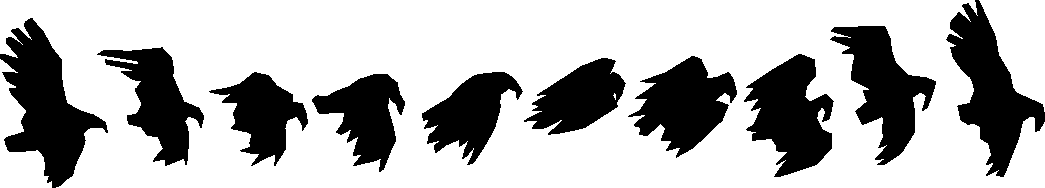
\includegraphics[scale=0.4, angle=20]{ptaki.pdf}
      }
      ;
    \node[yshift=1.0cm,xshift=0.6cm] (logopos) at (current page.south west) {{\begin{tikzpicture}\shuffleducks\duck[signpost=\insertframenumber, \randomhead,scale=.4]\end{tikzpicture}}};
    \pgfmathsetmacro{\progress}{360*(\insertframenumber)/(\inserttotalframenumber)};
    \draw[line width=0.2*3pt] ([xshift=0.55cm] logopos)  arc[radius=0.55cm, start angle=0, end angle=\progress];
    \fill ([shift={(\progress:0.55cm)}] logopos) circle(1pt);

    }
        \end{tikzpicture}
    
}

\newcommand{\SeMPowisko}{%
\large S\normalsize%
\kern-.3em \lower.2ex\hbox{e}%
\lower.2ex\hbox{\large M\normalsize}%
\kern-.1em \raise.1ex\hbox{\large P\normalsize}%
\kern-.3em \lower.2ex\hbox{o}%
\kern-.2em \raise.2ex\hbox{w}%
\lower.2ex\hbox{i}%
s%
\raise.2ex\hbox{k}%
\kern-.3em \lower.2ex\hbox{o}%
}

\setbeamerfont{caption}{size=\tiny}

\title[Papier w zastosowaniach elektronicznych i~optoelektronicznych$^1$]{Papier w zastosowaniach elektronicznych i~optoelektronicznych\footnote{sygnały optyczne $\leftrightarrow$ sygnały elektroniczne}}
% \subtitle{Przegląd niektórych eksperymentów}
\author[M. Winiarski]{Mateusz Winiarski}
\institute[fizyk UJ]{fizyka IV-I, WFAIS}
\date[dzisiaj]{13 maja 2024\\dzisiaj}

\begin{document}

\frame{\titlepage}

\section{Papier}
        \begin{frame}{Wady \hfill i \hfill zalety}
\begin{columns}

\begin{column}{0.5\textwidth}
    \begin{itemize}
        \item zasadniczo nie przewodzi prądu
        \item jest nieprzezroczysty
        \item jest chropowaty
        \item jest porowaty i niewodoodporny
    \end{itemize}
\end{column}
\begin{column}{0.5\textwidth}
    \begin{itemize}
        \item jest tani (tańszy nawet niż plastik)
        \item jest łatwy w produkcji
        \item jest ekologiczny
        \item jest giętki
        \item zasadniczo nie przewodzi prądu
    \end{itemize}
    % \pause
    \end{column}
% \begin{column}{0.5\textwidth}
%     \begin{figure}
%         \centering
%         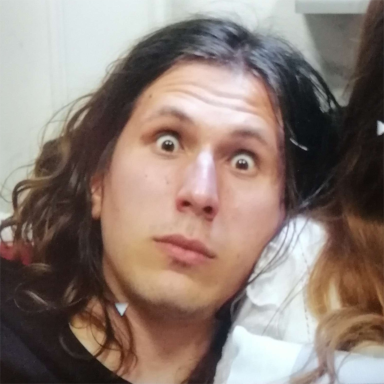
\includegraphics[width=0.9\linewidth]{firlejpatrzy.png}
%         \caption{Your reaction to that information}
%     \end{figure}
% \end{column}
\end{columns}
\end{frame}

\begin{frame}{Jak pozbyć się wad}
    
\end{frame}

\begin{frame}{Lista zastosowań}
\begin{tabular}{@{$\blacktriangleright$ }l @{$\quad\to\quad$ } l}
    fotowoltaika & pokrycia antyodblaskowe \\
    obwody elektroniczne & FETy, elektrolity \\
    ekrany & podłoża OLEDów i ekranów dotykowych \\
    magazynowanie energii & elektrody, separatory \\
    anteny & podłoża \\
\end{tabular}
\end{frame}


\section{Fotowoltaika}

\begin{frame}{Fotowoltaika}
    \begin{itemize}
        \item problem: utrata światła związana z odbiciem
        \item rozwiązanie: warstwy antyodblaskowe
    \end{itemize}
    \begin{columns}
        \begin{column}{0.5\textwidth}
            \begin{itemize}
            \item materiały:
            \begin{itemize}
                \item błony dielektryczne
                \item nanostruktury krzemowe
                \item materiały plazmoniczne
            \end{itemize}
            \end{itemize}
        \end{column}
        \begin{column}{0.5\textwidth}
            \begin{itemize}
            \item wady:
            \begin{itemize}
                \item wysoka cena
                \item właściwości silnie zależne od kąta padania lub długości fali
            \end{itemize}
            \end{itemize}
        \end{column}
    \end{columns}
\end{frame}

\begin{frame}{Jak to naprawić za pomocą papieru I}
    \begin{figure}[h]
        \centering
        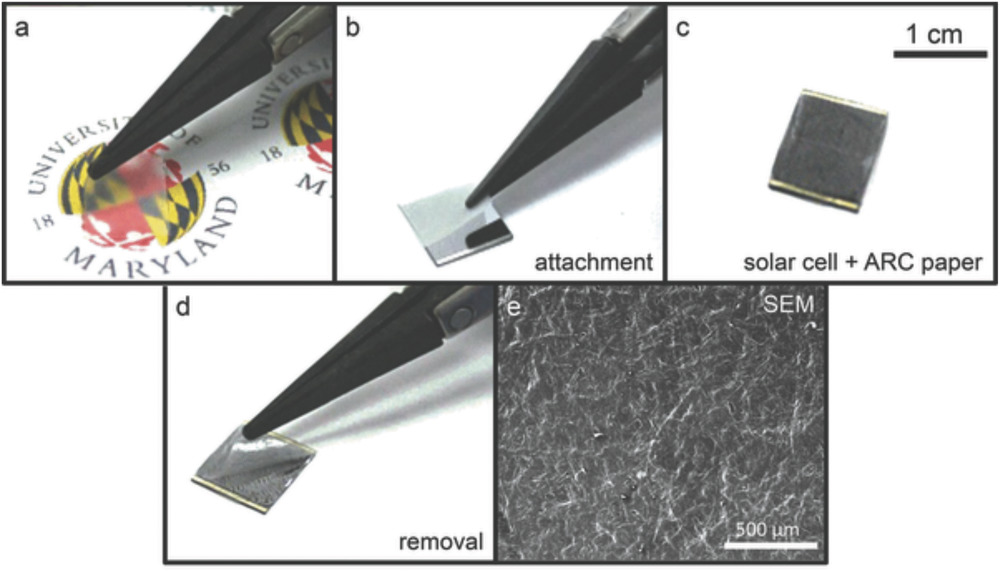
\includegraphics[width=0.75\linewidth]{fig2.png}
        \caption{a–c) Paper transfer and removal process. (a) The transparent cellulose paper used as an antireflection coating. (b) Transfer of the transparent paper antireflection coating on a GaAs solar cell. PVAc is used as a binding material. (c) The cell with the transparent cellulose paper antireflection coating on top. d) The paper can be removed as needed. e) A SEM image showing cellulose fibers within the transparent paper antireflection coating.\\
        \typeout{twoja stara sra do gara}
        [source: \url{https://doi.org/10.1002/aenm.201301804}]
        }
        % \label{fig:enter-label}
        
    \end{figure}

\end{frame}
\begin{frame}{Jak to naprawić za pomocą papieru II}
    \typeout{a twój stary to wpierdala}

    \begin{figure}[h]
        \centering
         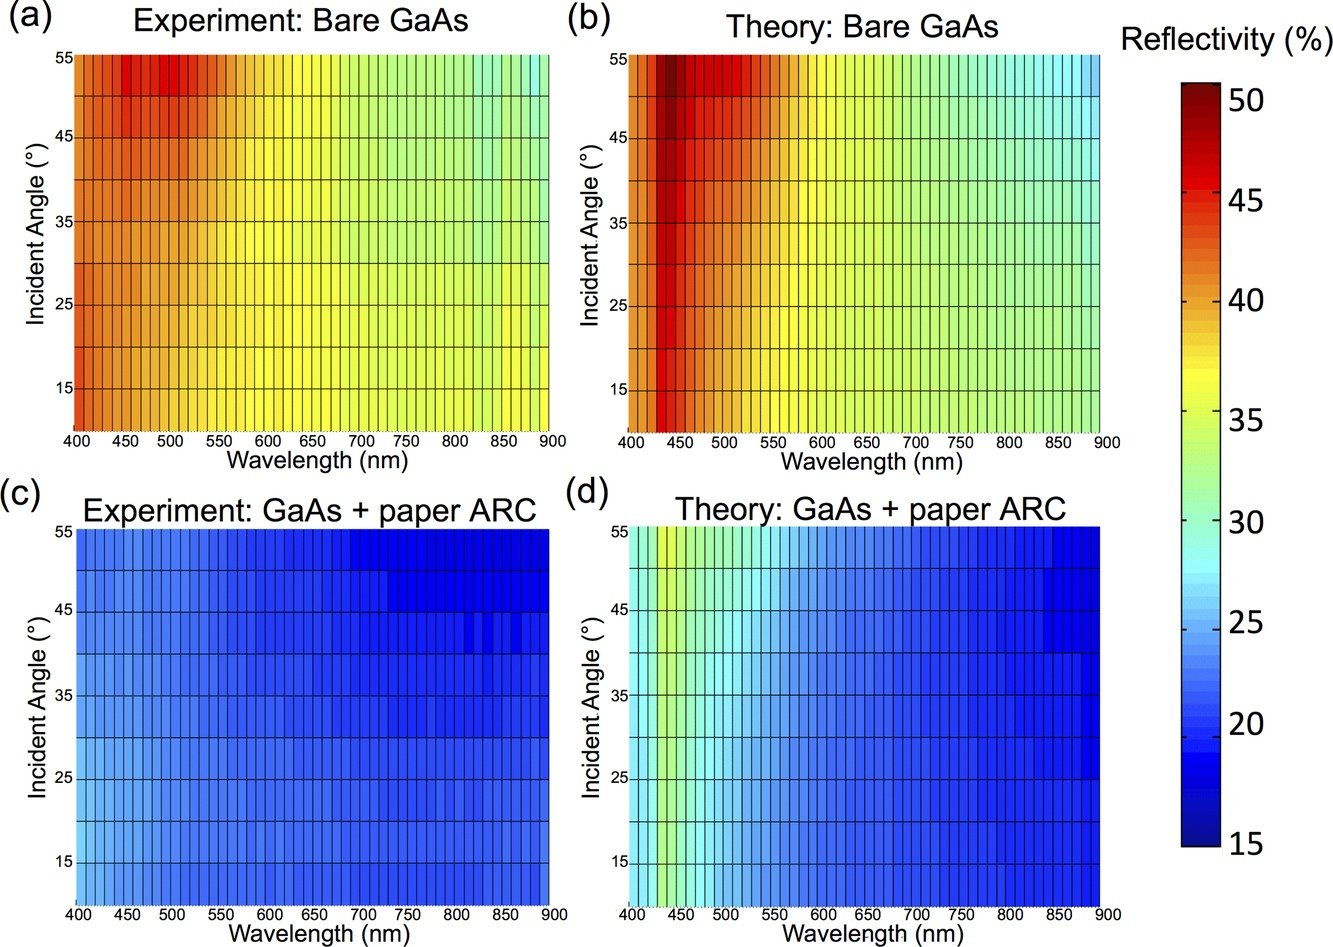
\includegraphics[width=0.65\linewidth]{fig3.png}
         \caption{
         Transparent paper ARC reduces reflection over a wide range of incident angles and wavelengths. For the bare GaAs cell, contour plots of a) measured and b) calculated reflectivity as a function of incident angle \typeout{dx}(from 10\si\degree to 55\si\degree)\typeout{xd} and wavelength (from 400 nm to 900 nm) are in close agreement. The addition of a transparent paper ARC greatly reduces the measured reflection (c) over all angles and wavelengths. Calculations using an incoherent reflection model accurately predict the expected reduction of the reflectivity (d). Differences between the experiment and the calculations near $\lambda$ = 430 nm are predominately due to differences in the optical properties of the GaAs used and are independent of the paper ARC.\\ \typeout{twoja stara to kopara}
	        [source: \url{https://doi.org/10.1002/aenm.201301804}]
         }
%         \label{fig:enter-label}
        \typeout{nasrałem}
    \end{figure}
\end{frame}


\section{Obwody elektroniczne}

\begin{frame}{Obwody elektroniczne}

\begin{itemize}
\item problem:
\end{itemize}
    
\end{frame}

\section{Magazynowanie energii}

\begin{frame}{Frame Title}
    
\end{frame}

\section{Anteny}

\begin{frame}{Frame Title}
    
\end{frame}

\section{Podsumowanie}

\begin{frame}{Frame Title}
    
\end{frame}

\begin{frame}{}

\begin{figure}

\centering
    \begin{tikzpicture}
      \duck[parrot, body=gray!30!yellow, head=gray!30!yellow, bill=red, tshirt=white!30!black, peakedcap=blue!50!black, ribbon=gray, bowtie=blue, crozier=brown!80!black]
      %\addwater{blue!50!cyan}
      \fill[cyan!20!white] (-1.4,1.8) ellipse (1.8 and 0.5);
  \fill[cyan!20!white] (-0.2,1.54) -- (0.2,1.35) -- (0.0,1.6) -- cycle;
	\node at (-1.4,1.8) {Dziękuję za uwagę};
    \end{tikzpicture}
    \end{figure}


    
    \begin{figure}
    \centering
    \qrcode[height=0.3\textwidth]{https://github.com/falcotinnunculus/przezrocza/tree/wladca/papier}\\
    {\tiny https://github.com/falcotinnunculus/przezrocza/tree/wladca/papier}

    \end{figure}
\end{frame}


% \appendix

% \begin{frame}{Współczynniki}
    
% \end{frame}

\end{document}